\documentclass{article}
\usepackage{sbaush-article}
\usepackage[italian]{babel}
\usepackage[utf8]{inputenc}
\usepackage{graphicx}
\usepackage{makeidx}
\usepackage{array}
\usepackage{tocbibind}
\usepackage{listings}
\usepackage{color}

%\usepackage[dvipsone]{color}[dvips,etc)  ;-)

\definecolor{Light}{gray}{.90}
%\definecolor{Dark{gray}{{.20}
\def\myComment#1{\colorbox{Light}{\parbox{\textwidth}{\emph{#1}}}}
\def\myCommentSpace#1{\vspace{0.5cm}\colorbox{Light}{\parbox{\textwidth}{\emph{#1}}}\vspace{0.5cm}}


\lecture{1}

\def\firstauthor{Nicola Martorana}
\def\secondauthor{Iacopo Masi}
\def\thirdauthor{Marco Meoni}
\def\coursenumber{ARC}
\def\class{Relazione di Analisi Immagini e Video}
\def\title{Comparazione di Kalman e ConDensation in video-tracking}
\def\semester{2006/2007}
\def\instructor{P. Crescenzi}
\def\date{Maggio 2007}
\def\professor{Prof. Pietro Pala}
\def\firstassistant{Ing. Walter Nunziati}
\def\secondassistant{Ing. Andy Bagdanov}

\begin{document}

\maketitle
\tableofcontents
\listoffigures
\lstlistoflistings
\section{Introduzione}
Questa relazione descrive lo studio effettuato, i metodi utilizzati ed i risultati raggiunti per la realizzazione dell'elaborato relativo al corso di Analisi delle immagini e dei video, appartenente al corso di laurea specialistica in Ingegneria Informatica di Firenze, tenuto dal Prof. Pietro Pala.

L'elaborato si è incentrato sullo studio di due algoritmi di \textit{tracking} video, il filtro di Kalman ed il ConDensation, iniziando con l'approfondimento delle rispettive basi teoriche per poi passare all'implementazione di entrambi, finalizzata all'ottenimento di risultati comparativi, che sono stati catalogati ed interpretati. Lo sviluppo dell'elaborato è stato coordinato all'interno del \textit{Media Integration and Communication Center}\footnote{MICC, http://www.micc.unifi.it/} in particolare dall'Ing. Walter Nunziati e dall'Ing. Andrew D. Bagdanov, ai quali va un particolare ringraziamento per l'attenzione che hanno riposto in questo lavoro.
\begin{figure}[hb]
\centering
	
\includegraphics[scale=0.6]{micc.png}
\caption{\textit{Media Integration and Communication Centre, Firenze}\label{fig:micc}}
\end{figure}

L'implementazione del software che ha fornito i risultati comparativi è stata effettuata nel linguaggio di programmazione C++ tramite le librerie per il computer vision OpenCV\footnote{Open Source Computer Vision Library http://www.intel.com/technology/computing/opencv/}, sviluppate internamente ad Intel, ma rese pubblicamente fruibili ed utilizzabili tramite una licenza \textit{GPL-compatibile}; lo sviluppo del codice è stato effettuato sotto controllo di versione Subversion (SVN), in hosting presso Google Code\footnote{http://code.google.com/p/video-tracker/}. Il software è stato reso pubblico sotto licenza libera GNU GPL\footnote{GNU General Public License http://www.gnu.org/licenses/gpl.html}.

Grazie al sistema di controllo di versione è stato possibile sviluppare il software contemporaneamente sia sotto architettura Unix (nello specifico diverse distribuzioni di GNU/Linux) che sotto architettura Microsoft Windows, risultando così pienamente compatibile con entrambe.

Con questa relazione ci si prefigge l'obiettivo di ripercorrere il cammino fatto nello sviluppo dell'elaborato, iniziando nel primo capitolo con una introduzione ai due metodi di \textit{tracking}, con un breve approfondimento delle rispettive basi matematiche per poi concludere focalizzando l'attenzione sulla specifica implementazione del modello utilizzato.

La descrizione passerà nel secondo capitolo ad affrontare lo sviluppo del software che ha reso possibile lo sviluppo della comparazione, approfondendo i punti fondamentali delle librerie utilizzate per andare poi ad analizzare dettagliatamente il \textit{control-flow} del programma. 

L'ultima sezione sarà invece dedicata allo studio dei risultati ottenuti, e fornirà i risultati più importanti di tutta la serie di esperimenti che sono stati compiuti con il software ottenuto, riportandone grafici comparativi e schermate di esecuzione.

%Rapida descrizione dell'elaborato e di come si articola la relazione, motivazioni della ricerca ecc...
\section{Metodi di tracking basati su modelli}
Il \textit{video tracking} è il processo secondo il quale si localizza un oggetto in movimento all'interno di uno stram video e rappresenta uno dei più interessanti problemi di \textit{computer vision}. Esistono svariati approcci al video tracking, ognuno orientato ad ottimizzare le prestazioni relativamente al campo d'azione. In questo lavoro è stata effettuata la scelta di effettuare il tracking secondo l'approccio basato su modelli, che viene eseguito secondo due passi fondamentali: la localizzazione dell'oggetto da tracciare ed il tracciamento effettivo.

Il primo passo, computazionalmente non molto oneroso, è stato realizzato tramite il \textit{background subtraction} (descritto nella sezione ???) e consiste nella rilevazione dell'oggetto all'interno dell'immagine e nell'ottenimento delle informazioni relative.

Il secondo passo, ovvero l'applicazione del tracking al video, rappresenta il punto di maggior interesse del lavoro in quanto consiste nell'elaborazione di una stima della posizione al frame successivo dell'oggetto selezionato; l'esecuzione si basa sull'elaborazione dei dati ottenuti dal processo di localizzazione dell'oggetto.

Gli obiettivi di questo elaborato sono la realizzazione, l'analisi e la comparazione dei due più importanti algoritmi di tracking basato su modelli: il filtro di Kalman, descritto nella sezione \ref{kalman} ed il Condensation, descritto nella sezione \ref{condensation}.

\textbf{Questa parte va espansa mettendo un po' di discorsi sul tracking generale e poi andando a parare sul tracking model based}

\subsection{Kalman Filter}\label{kalman}
Il Kalman Filter\cite{kalman-intro} è un efficiente filtro ricorsivo che valuta e stima lo stato di un sistema dinamico sulla base di una serie di misure soggette a rumore. Il filtro è molto potente in quanto supporta la stima degli stati passati, presenti e futuri del sistema anche quando la natura del sistema è sconosciuta. \'E usato in molti campi ingegneristici, che vanno dall'applicazione in tecnologie radar all'applicazione in computer vision, come utilizzato in questo stesso ambito.
\subsubsection{Definizione del modello}
Il filtro ha l'obiettivo di stimare lo stato $x \in \Re^n$ di un processo a tempo discreto governato dalla seguente equazione alle differenze
\begin{equation}\label{eq:x}
 x_k=Ax_{k-1}+Bu_{k-1}+w_{k-1}
\end{equation} 
dove 
\begin{description}
 \item [$A$] è la matrice di transizione del modello, ed è applicata allo stato precedente $x_{k-1}$; è quindi una matrice quadrata che mette in relazione due vettori delle stesse dimensioni: lo stato al tempo $k-1$ e lo stato al tempo $k$. Risulta la responsabile dell'aggiornamento dello stato.
\item [$B$] è la matrice di controllo sull'input del sistema. \'E applicata al vettore di controllo $u_{k-1} \in \Re^l$ e mappa questo nella dimensione dello stato $x$; è quindi una matrice rettangolare $nxl$.
\item [$w_k \in \Re^n$] è il rumore che affligge il processo. Si assume che sia descritto da una gaussiana a media $0$ e covarianza descritta dalla matrice $Q_k$. Formalmente $w_k \sim N(0,Q_k)$.
\end{description}

Al tempo $k$ l'osservazione dello stato reale $x_k$ è effettuata tramite il vettore della misura $z \in \Re^m$ che è modellato da
\begin{equation}\label{eq:z}
z_k=Hx_k+v_k
\end{equation}
dove 
\begin{description}
 \item [$H$] è la matrice che mappa lo spazio dello stato reale nello spazio dello stato osservato e risulta per questo rettangolare, di dimensione $mxn$.
\item [$v_k \in \Re^m$] è il rumore dell'osservazione, che come per il rumore $w_k$ è descritto da una gaussiana a media zero e covarianza $R_k$. Formalmente si può esprimere come $v_k \sim N(0,R_k)$.
\end{description}
 Da notare che lo stato iniziale ed i vettori che descrivono la presenza di rumore negli stati successivi sono da considerarsi mutualmente indipendenti.

Come detto in precedenza il filtro di Kalman è un estimatore ricorsivo: questo significa che il filtro applica la sua stima dello stato del processo ed ottiene un feedback nella forma del vettore della misura, dal quale può aggiornare la sua computazione. 

Le equazioni del filtro sono raggruppabili in due macrocategorie: \textit{time-update}, responsabili della proiezione nel tempo dello stato corrente per ottenere la stima a prori dello stato successivo (rappresentata dal vettore $\hat{x}_k^- \in \Re^n$), e \textit{measurement-update}, responsabili dell'incorporazione della misura allo stato corrente nella stima a priori, ottenendo così la stima a posteriori (rappresentata dal vettore $\hat{x}_k \in \Re^n$). 

Solitamente lo stadio relativo al \textit{time-update} viene definito come \textit{predict}, mentre quello relatico al \textit{measurement-update} come \textit{correct}.

\begin{figure}[hb]
\centering
	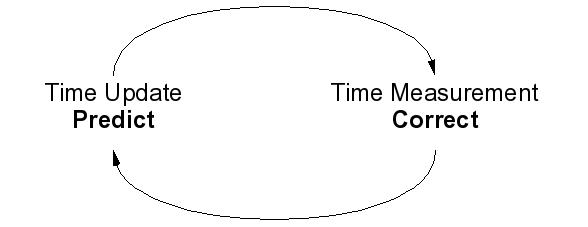
\includegraphics[scale=0.3]{PredCorr.jpg}
\caption{\textit{Il ciclio di calcolo del filtro di Kalman.}\label{fig:predictcorrect}}
\end{figure}
\subsubsection{Predict}
Le equazioni specifiche per il passo di \textit{predict}, che proiettano lo stato e la covarianza dallo stato $k-1$ allo stato $k$ sono 
\begin{equation}\label{eq:prior}
\hat{x}_k^-=A \hat{x}_{k-1}+Bu_{k-1}
\end{equation} 
\begin{equation}
P_k^-=A P_{k-1}A^T+Q
\end{equation} 
dove $A$ e $B$ derivano dalla formula (\ref{eq:x}), considerando sempre la covarianza relativa a $w$ come $Q$, mentre $P_k^-$ è una matrice che rappresenta la covarianza sull'errore nella stima a priori e $P_k$ è una matrice che rappresenta la covarianza sull'errore nella stima a posteriori.
\subsubsection{Correct}

Le equazioni che invece formalizzano il passo di \textit{correct} effettuano una stima sul guadagno del filtro tra l'osservazione attuale e quella predetta (\ref{eq:K}), ottengono la stima a posteriori  (equazione (\ref{eq:post})) data la stima a priori effettuata nel passo di update (\ref{eq:prior}) e dall'osservazione dello stato reale, definita in \ref{eq:z}; viene calcolata anche la covarianza sull'errore nella stima a posteriori (\ref{eq:P}):
\begin{equation}\label{eq:K}
K_k = P_k^- K_T(HP_k^-H^T+R)^{-1}
\end{equation} 

\begin{equation}\label{eq:post}
\hat{x}_k=\hat{x}_k^-+K_k(z_k-H\hat{x}_k^-)
\end{equation} 

\begin{equation}\label{eq:P}
P_k=(1-K_kH)P_k^-
\end{equation} 

\subsubsection{Parametri e configurazione del filtro}
L'esecuzione dell'algoritmo è direttamente dipendente dalla scelta che viene effettuata riguardo ai parametri 
\begin{figure}[hb]
\centering
	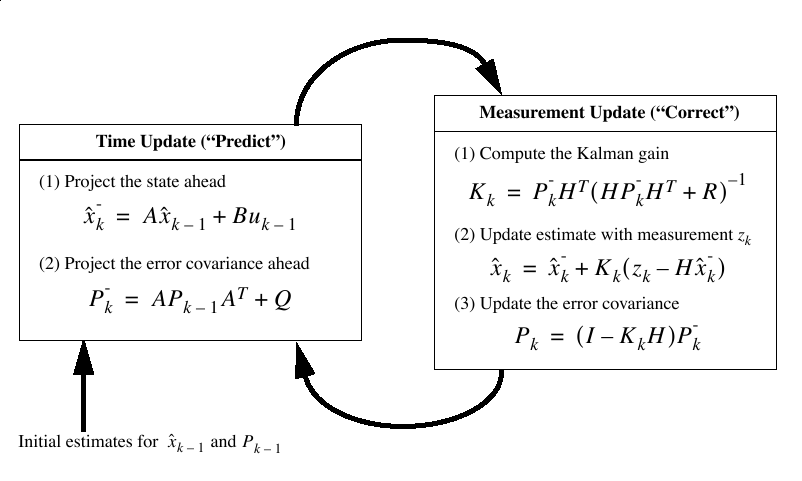
\includegraphics[scale=0.4]{cicloKalman.png}
\caption{\textit{Ciclo di Kalman completo, con parametri ed equazioni}\label{fig:completeKalman}}
\end{figure}
\subsection{ConDenSation}\label{condensation}
\textbf{descrivere seriamente il particle filter (tipo dagli articoli o dalla wiki) mettendo anche dettagli matematicosi}

\subsection{Descrizione dell' implementazione dei modelli}
Fare cappello su cosa è un modello poi particolareggiare verso il nostro modello

QUESTA PARTE VA FATTA BENE

ricordarsi di mettere la descrizione del background subtraction per quanto riguarda il ruolo dell'oggetto.

come sono fatte le matrici che descrivono 
dire che noi s'ha un generico sistema descritto unicamente dalla sua posizione sul piano e dalla sua velocità orizz e verticale

Cosa si prende per varianza di uno dell'altro, come è fatto lo stato (vettore i 4 dimensioni di cui 2 posizione xy etc..)

     %%%%%%%%%%%%%%%%%%%%
     %                  %
     %  capitolo1.tex   %
     %                  %
     %%%%%%%%%%%%%%%%%%%%

\section{Sviluppo dell'applicativo}

\subsection{Obiettivi}
L' obiettivo del software è quello di realizzare un applicativo che esegua \textit{model based tracking} \ref{modelTracking} sulla base di un video passatogli come ingresso. Più nel dettaglio l'applicazione esegue il tracciamento tramite il filtro di Kalman \cite{kalman-intro} e il ConDensaTion \cite{kalman-condense}, in maniera tale da poter confrontare le prestazioni dell' uno e dell'altro.\\
Altri requisiti funzionali sono quelli di:

\begin{itemize}
 \item  fare scegliere all'utente l'oggetto da tracciare in caso di tracking multiplo: in questo caso il software si ferma sul primo frame del video, dando possibilità di scegliere l'oggetto di cui si vuol fare il tracciamento. Per migliorare la selezione di un oggetto, vengono evidenziati dei un puntini gialli in corrispondenza del blob identificato. Vedi figura \ref{fig:scelta2blob}

\item tracciare a video l'andamento dei due algoritmi, evidenziandoli con colori differenti; visualizzare un' ellissi per ogni algoritmo che indichi la varianza del vettore di stato per quel tipo di tracking.

\item fornire un output razionalizzato su terminale e su filesystem per verificare rispettivamente la corretta esecuzione degli algoritmi e per avere un riscontro finale sulle performance e l'accuratezza di ognuno. Successivamente parsare i suddetti file per una rappresentazione grafica dell'accuratezza dei due metodi di tracking.

\item progettare e realizzare l'applicazione in maniera tale che possa essere compilata ed eseguite su piattaforme diverse.


\end{itemize}

I dettagli implementativi di questi punti sono rimandati alla sottosezione  \ref{ControlFlow}

\begin{figure}[hb]
\centering
	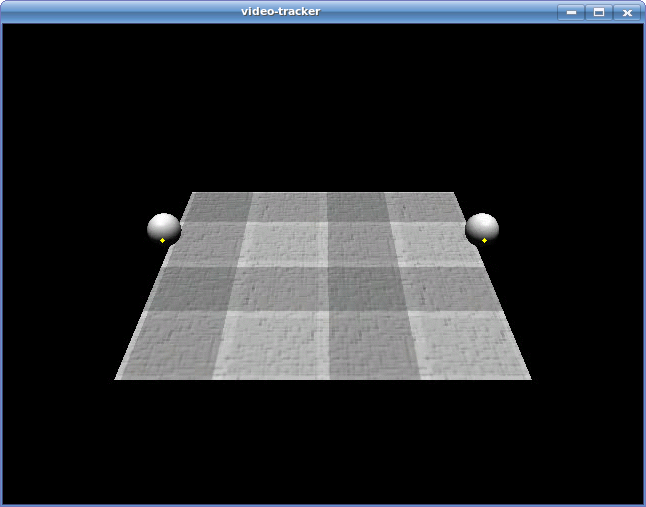
\includegraphics[scale=0.5]{doppiascelta.png}
\caption[Esempio di scelta tra due blob]{\textit{Esempio di scelta tra due blob su tracking multiplo: l'utente ha la possibilità di sccegliere su quale blob effettuare il tracciamento semplicemente cliccando vicino ad uno dei punti gialli. Il Sistema automaticamente selezionerà il blob più vicino attraverso il calcolo della distanza euclidea}\label{fig:scelta2blob}}
\end{figure}


\'E bene sottolineare che il video in ingresso possiede delle restrizioni: infatti affinchè il \textit{background subtraction} lavori in maniera ottima, è necessario che il video:
\begin{itemize}
 \item possieda semper uno sfondo fisso o che comunque non vari durante la ripresa. Cambiare sfondo sarrebbe come rinizializzare l'agoritmo per il detecting dei blob.
\item possieda un numero ( $n > 40 $ ) di frame inziale che mostrino solo il background per facilitare il calcolo della \textit{ground truth}, cioè del blob osservato da cui prendere le misure per i due algoritmi.
\item sia stato registrato da una postazione fissa e quindi che la telecamera di ripersa non introduca nel video un moto relativo.
 \end{itemize}

Qualsiasi video che rispetta questi tre vincoli è considerato non solo adeguato, ma ottimale per effettuare il tracking con la nostra applicazione.




%ingresso video fatto in un certo modo (sfondo fisso, tot frame di background iniziale, telecamera fissa)

%uno o + oggetti in moto

%permette di selezionare QUALE oggetto seguire, farne il tracciamento reale, ottenere le predizioni secondo k e c, e raccoglierne dati e risultati per la realizzazione di grafici

%intro utilizzo librerie utilizzate intel openCV
\subsection{Librerie Intel OpenCV}
Per svilluppare l'applicazione sono state utilizzate le libreria \textit{OpenCV}, emergente nel campo della \textit{computer vision}  e sviluppata da Intel sotto una licenza di tipo OpenSource, compatibile con la GNU GPL.
\'E bene però prima fare chiarezza sull'uso e lo scopo di queste librerie.\\
La capacità di interpretare ed utilizzare correttamente le informazioni acquisite da una videocamera o fotocamera attualmente presenta molti problemi insoluti. Convertire un’immagine in informazioni “oggettive” astraendone il contenuto dalla pura rappresentazione luminosa, sebbene sia un’operazione banale per un cervello umano adulto è, a tutt’oggi, un problema di elevata complessità per un sistema automatico.
Oltretutto il campo di ricerca è evidentemente molto giovane, con meno di trent’anni di esperienza. In quest’ottica si inserisce la necessità di una base comune di potenti strumenti analitici, primo dei quali una \textbf{libreria} che raccolga le funzionalità degli algoritmi più utilizzati e citati in letteratura, oltre che una serie di formati di rappresentazione dei dati secondo standard aperti e condivisi.\\
Le librerie OpenCV (Open Source Computer Vision) nascono appunto a questo scopo; lo sviluppo prende le mossa da un gruppo di ricerca sponsorizzato da Intel. E’ infatti parzialmente basata sulla \textit{Intel Image Processing Library (IPL)}: tale prodotto è oggi integrato nella libreria commerciale IIPP (Intel Integrated Performance Primitives), con cui conserva piena compatibilità e che può eventualmente rendere disponibili un completo ventaglio di funzioni più specifiche.\\
Tra i punti di forza sottolineiamo inoltre la politica di licenza utilizzata, in stile BSD e definita nella ``Intel License Agreement For Open Source Computer Vision Library'', completamente compatibile con la licenza GPL. A grandi linee questo permette una libera ridistribuzione sia in forma sorgente che binaria, anche all’interno di prodotti commerciali, a condizione di mantenere le note di copyright e di non utilizzare il nome Intel a scopo promozionale di prodotti derivati.\\
Inoltre un' altra potenzialità offerta è la caratteristica di essere \textit{cross-platform}: cioè possono essere compilate e usate sia sotto sistema operativo Microsft Windows che GNU/Linux. Questa caratteristica le rende molto appetibili per i requisiti di portabilià che ci eravamo prefissi di raggiungere.\\ Da notare che le librerie sono scritte in linguaggio C e non fanno uso quindi di un linguaggio orientato agli oggetti.

\subsubsection{Aree funzionali delle librerie}
Si vuol chiarire subito un fatto che può essere causa di equivoci: con il termine ``libreria grafica'' infatti si identificano genericamente almeno tre famiglie di librerie, i cui scopi sono sostanzialmente differenti:
\begin{enumerate}
 \item  I Toolkit, ovvero librerie di primitive per la creazione di oggetti grafici di interfaccia (finestre, icone, bottoni,ecc). Parzialemente ricoperto in OpenCV dalle HighGui.
\item Librerie di rendering e multimedia, come DirectX e OpenGL, orientate alla massima performance nella creazione di effetti poligonali o vettoriali. L’utilizzo più comune è teso all’ottenimento di elevate prestazioni    grafiche sfruttate ad esempio nei videogiochi o nelle applicazioni multimediali.
\item  Librerie di gestione hardware grafico, come digitalizzatori e frame-grabber. Pur includendo tipicamente una base di funzioni di trattamento sono generalmente da considerarsi come API dei relativi driver hardware.
\end{enumerate}

Le OpenCV, pur includendo alcune funzionalità tipiche di ciascuna delle famiglie citate \footnote{vedi esempio delle HighGui}, non fanno parte di nessuno di questi gruppi. L’utilizzo primario è infatti quello collegato alla visione artificiale, il cui problema principale, come già visto, è quello di estrarre da immagini/video dati significativi, trattabili in modo automatico. Tale campo di studio trova le sue applicazioni più comuni nella robotica, nei sistemi di  videosorveglianza evoluti e nei sistemi di monitoraggio e sicurezza, oltre che in ogni sistema di archiviazione automatica di informazioni visive.\\
La libreria include attualmente più di 300 funzioni, che coprono le più svariate esigenze di trattamento di immagini, comprese funzioni matematiche ottimizzate (elevamento a potenza, logaritmi, conversioni cartesiane-polari, ecc.) ed  un completo pacchetto di algebra matriciale, sviluppato funzionalmente al resto del sistema.\\

La principale categoria di uso rimane comunque il processing di tipo real-time su immagini e video. \\
Una panoramica generale delle librerie comprende questi aspetti della computer vision:
\begin{enumerate}
\item Human-Computer Interface (HCI)
\item Object Identification
\item Segmentation and Recognition
\item Face Recognition e Gesture Recognition
\item Motion Tracking  riferimento al nostro progetto
\end{enumerate}

%descrivere un po queste aree e dove si usano noi nel nostro progetto.




\subsubsection{Riferimenti}

Come molti progetti opensource in maturazione \footnote{La versione 1.0 ufficiale è stata rilasciata nel tardo 2006; parte del progetto è stato scritto con librerie in beta testing} è stata carente la parte che riguarda la documentazione. Nonostante la presenza di un colosso alla spalle e di una struttura basata sul modello wiki, la documentazione ufficiale in pdf e html, anche se facilmente fruibile, non è stata sufficiente per colmare le lacune iniziali. Per questo motivo è stato effettuato un grosso lavoro di studio per capire il funzionamento del toolkit OpenCv, che spesso è terminato con la ricerca di documentazione in website asiatici, dove sembra che queste librerie siano molto gradite.\\
Alcuni riferimenti importanti per OpenCV:
\begin{itemize}
 \item \htmladdnormallink{Sito web ufficiale}{http://www.intel.com/technology/computing/opencv/index.htm}
\item \htmladdnormallink{Portale di wiki}{http://opencvlibrary.sourceforge.net}
\item \htmladdnormallink{ OpenCv - Groups Community}{http://tech.groups.yahoo.com/group/OpenCV/}
\end{itemize}

 
\subsection{Control Flow del programma}\label{ControlFlow}
%intro del ciclozzo FOR e che cosa viene fatto in ordine con l'acquisizione frame/frame del video
Come citato precedentemente, si va ora a evidenziare quelli che sono stato gli accorgimenti tecnici per implementare il nostro software di comparazione tra Kalman e Condensation.\\
Si cercherà di non riportare tutto il codice sorgente, ma di evidenziare solo spezzoni di esso, che possono fornire preziose informazioni sulla struttura. \'E bene sottolineare che in linea con le OpenCV, la parte principale del software non è stata sviluppata secondo il paradigma Object Oriented, ma si è usato la razionalizzazione delle strutture dati in classi solo quando necessario.
Il nucleo centrale dell' applicazione è il \textbf{ciclo for} che dipende dalla lunghezza del video da analizzare. Ogni calcolo verrà fatto quindi in \textbf{modalità online}, cioè ad ogni passo dentro il ciclo stesso. Ne listato di pseudo codice sottostante è riprotato l'idea dell' andamento dell'applicativo. 
\newpage

\lstset{language=c++}
\lstset{commentstyle=\emph}
\begin{lstlisting}[frame=l,caption=Nucleo dell'Applicazione - execute.cpp ,breaklines=true,basicstyle=\small]{Nucleo dell'Applicazione - execute.cpp}

void execute( file ){

	video = captureFromAvi( file )
	
	initBackgroundSubtraction( video )

	for( int fr = 1; frame = captureNextFrame( video ), fr++ ){
	
		updateBackgroundSubtraction( frame )
		
		if ( frame == FIRST_FRAME){
			
			blobs = getBlobSelectedFromUser( frame )
	
			initKalman( blobs );
			
			initCondensation( blobs );
		}
	
		updateKalman();
		updateCondensation();
	}
}

\end{lstlisting}

\subsubsection{Back subtraction}
%realizzazione online del backsub, librerie eccetera
\subsubsection{Predizione}
\subsubsection{Rappresentazione della predizione}
\subsubsection{HiGui}
\subsubsection{Scripting GNUPlot}


     %%%%%%%%%%%%%%%%%%%%
     %                                                   %
     %  capitolo1.tex   %
     %                  %
     %%%%%%%%%%%%%%%%%%%%

\section{Esperimenti}\label{sec:esperimenti}

Il software prodotto è stato testato su molteplici video, tra i quali ne sono stati selezionati tre che si distinguevano per le condizioni di esecuzione, in particolare stimolando caratteristiche specifiche dei due algoritmi di tracking, in modo da efatizzarne i risultati. I tre filmati sono caratterizzati da una ripresa a camera fissa, con un singolo oggetto in movimento che può sia uscire dall'inquadratura che nascondersi dietro qualche ostacolo all'interno della scena (occlusione). 

In ognuno dei tre filmati i primi frames sono di solo sfondo, ovvero non compare alcun oggetto in moto; questa scelta è stata effettuata per facilitare l'applicazione del Background Subtraction.\\

Per ciascun video abbiamo osservato/confrontato il comportamento dei due filtri al variare di alcuni parametri quali:
\begin{itemize}
\item frequenza di campionamento (MOD)
\item covarianza relativa al rumore del processo studiato (Q) (stabilisce la tolleranza consentita alla predizione del filtro di Kalman)
\item numero di campioni utilizzati dal Condensation\\
\end{itemize}

I risultati prodotti per ciascuna prova sono rappresentati in due grafici:
\begin{itemize}
\item Il primo rappresenta per ogni campionamento:
\begin{itemize}
\item la posizione dell'oggetto
\item la posizione predetta dal filtro di Kalman
\item la posizione predetta dal Condensation
\end{itemize}
\item Il secondo rappresenta per ogni campionamento di quanto rispettivamente ciascuna predizione si discosta dalla posizione reale dell'oggetto.
\end{itemize}

Inoltre per ogni test viene dato il valore medio della distanza (in pixels) tra posizione predetta e posizione reale, sia per il filtro di Kalman \begin{math}(\bar \delta_K)\end{math} che per il Condensation \begin{math}(\bar \delta_C)\end{math}, oltre al valore della varianza media per il Condensation \begin{math}(\sigma_x,\sigma_y)\end{math}.


\newpage

\subsection{Video: movies12.mjpeg}\label{sec:video-occ}
\begin{itemize}
\item risoluzione: 640x480
\item fps: 25.00
\item durata: 50.4 s
\end{itemize}

\begin{figure}[hb]
\centering
	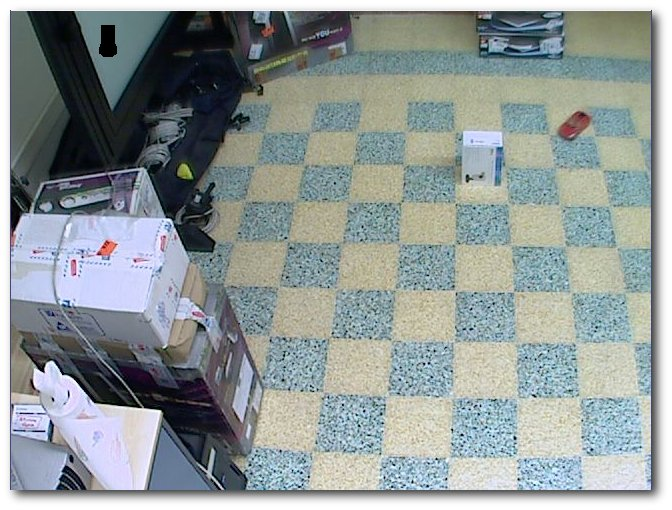
\includegraphics[scale=0.5]{movie12.jpg}
\caption{\textit{movie12 screenshot}}
\end{figure}

Si tratta di una ripresa trasversale dall'alto di un automobilina radiocomandata. In questa scena i punti di occlusione sono due: una scatola al centro della scena e un ostacolo sulla sinistra. La macchina non subisce repentine accelerazioni o decelerazioni, in generale ruota attorno alla scatola centrale e riamane nascosta dietro questa per un po'. L'automobilina non esce mai dalla scena.

%\begin{figure}[hb]
%\centering%
%	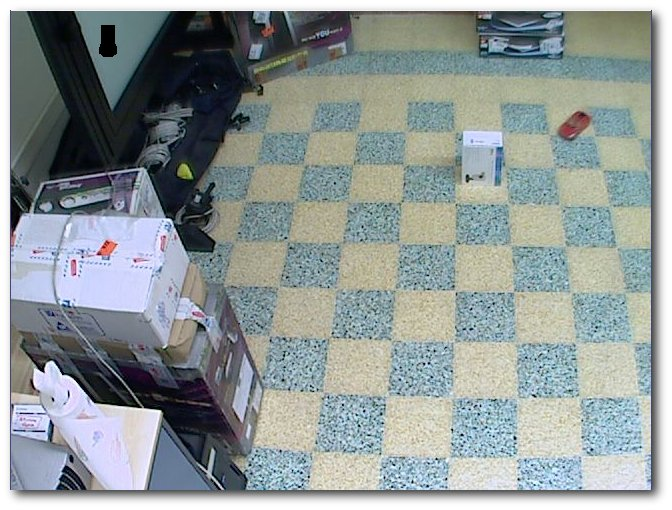
\includegraphics[scale=0.5]{movie12.jpg}
%\caption{\textit{movie12 screenshot}}
%\end{figure}
 
\newpage
\subsubsection{Test 1: MOD=3 , Q=1000, S=1000}

\begin{figure}[hb]
\centering
	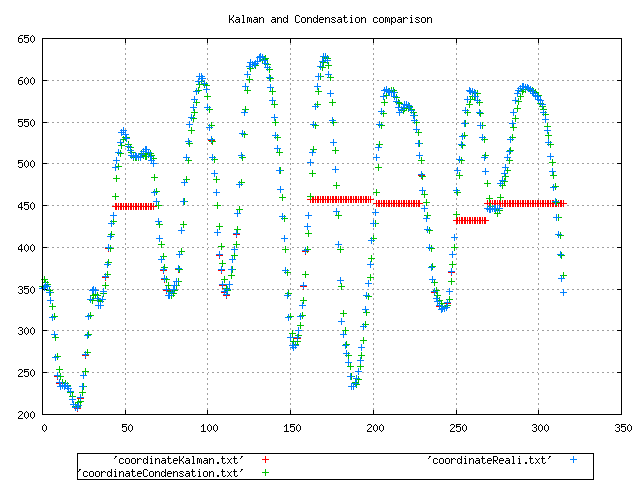
\includegraphics[scale=0.4]{../../esperimenti/movie12/mod_3-Q_1000-S_1000/plot.png}
\caption{\textit{Test 1: Tracciamento}}
\end{figure}

\begin{figure}[hb]
\centering
	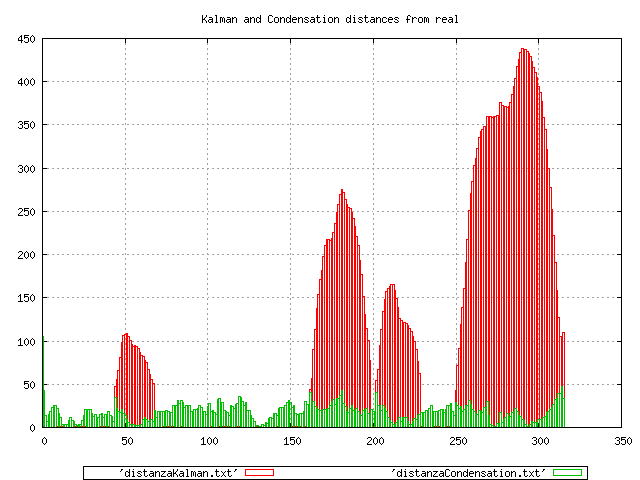
\includegraphics[scale=0.4]{../../esperimenti/movie12/mod_3-Q_1000-S_1000/plot-distances.png}
\caption{\textit{Test 1: Previsioni}}
\end{figure}

Statistiche:
\begin{itemize}
\item \begin{math} \bar \delta_K: 105 \end{math}
\item \begin{math} \bar \delta_C: 18 \end{math}
\item \begin{math}(\sigma_x,\sigma_y)\end{math}: (112,81)
\end{itemize}

Appare evidente che con queste impostazioni il filtro di Kalman non è in grado di mantenere traccia correttamente dell'oggetto, poichè più di una misurazione è persa a causa dell'occlusione. L'area di tolleranza per Kalman non è sufficiente. Tuttavia non appena l'oggetto ripassa vicino a dove Kalman si è fermato, questo ricomincia ad essere tracciato correttamente. Differentemente il Condenstaion non perde mai l'oggetto, ma la stima del moto è decisamente meno precisa.

\newpage

\subsubsection{Test 2: MOD=3, Q=2000, S=1000}

\begin{figure}[hb]
\centering
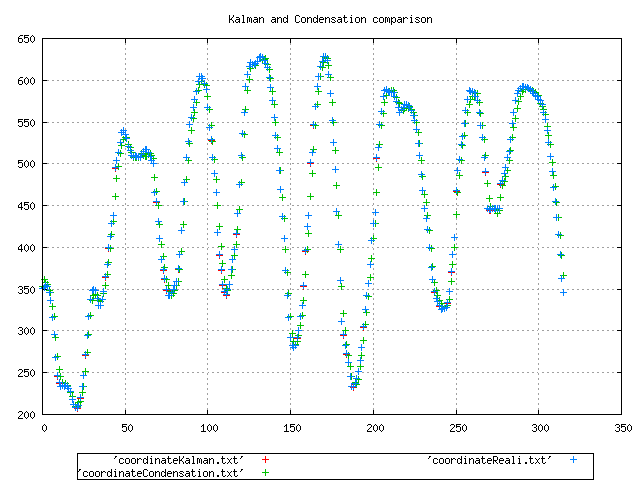
\includegraphics[scale=0.4]{../../esperimenti/movie12/mod_3-Q_2000-S_1000/plot.png}
\caption{\textit{Test 2: Tracciamento}}
\end{figure}

\begin{figure}[hb]
\centering
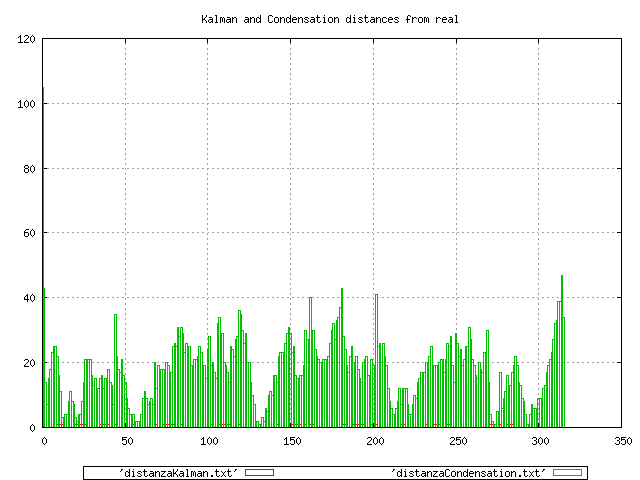
\includegraphics[scale=0.4]{../../esperimenti/movie12/mod_3-Q_2000-S_1000/plot-distances.png}
\caption{\textit{Test 2: Previsioni}}
\end{figure}

Statistiche:
\begin{itemize}
\item \begin{math} \bar \delta_K: 0 \end{math}
\item \begin{math} \bar \delta_C: 18 \end{math}
\item \begin{math}(\sigma_x,\sigma_y)\end{math}: (112,81)
\end{itemize}

Allargando l'area di confidenza per Kalman l'oggetto non viene mai perso e il tracciamento risulta pressochè perfetto. Il comportamrento in questo caso è evidentemente migliore del Condesation. Purtroppo un'area di confidenza troppo ampia potrebbe in alcune circostanze far perdere di validità al tracciamento. 

\newpage
\subsubsection{Test 3: MOD=3, Q=1000, S=5000}

\begin{figure}[hb]
\centering
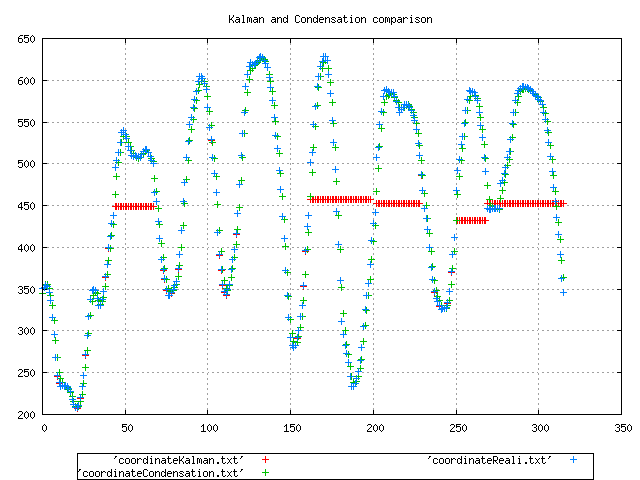
\includegraphics[scale=0.4]{../../esperimenti/movie12/mod_3-Q_1000-S_5000/plot.png}
\caption{\textit{Test 3: Tracciamento}}
\end{figure}

\begin{figure}[hb]
\centering
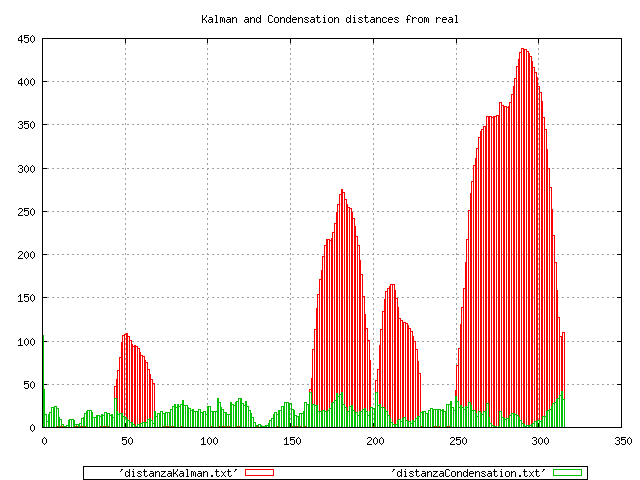
\includegraphics[scale=0.4]{../../esperimenti/movie12/mod_3-Q_1000-S_5000/plot-distances.png}
\caption{\textit{Test 3: Previsioni}}
\end{figure}

Statistiche:
\begin{itemize}
\item \begin{math} \bar \delta_K: 105 \end{math}
\item \begin{math} \bar \delta_C: 17 \end{math}
\item \begin{math}(\sigma_x,\sigma_y)\end{math}: (109,81)
\end{itemize}

Con questo test cominciamo a verificare il comportamento del Condensation alla variazione del numero di samples.
E' immediato osservare come aumentando il numero di samples da 1000 a 5000 questo non porti in media nessun significativo miglioramento.

\newpage
\subsubsection{Test 4: MOD=3, Q=1000, S=100}

\begin{figure}[hb]
\centering
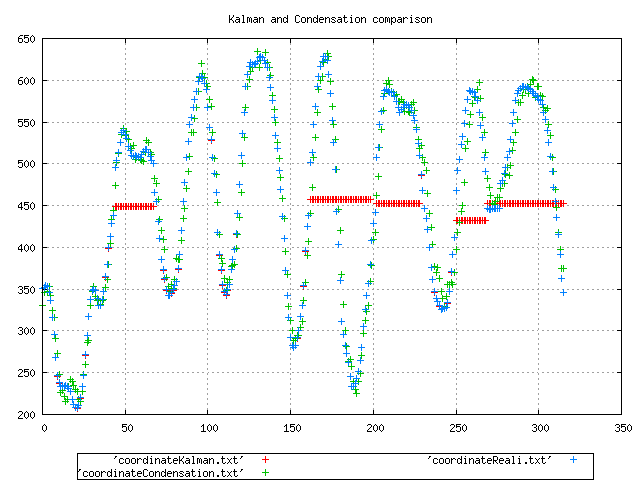
\includegraphics[scale=0.4]{../../esperimenti/movie12/mod_3-Q_1000-S_100/plot.png}
\caption{\textit{Test 4: Tracciamento}}
\end{figure}

\begin{figure}[hb]
\centering
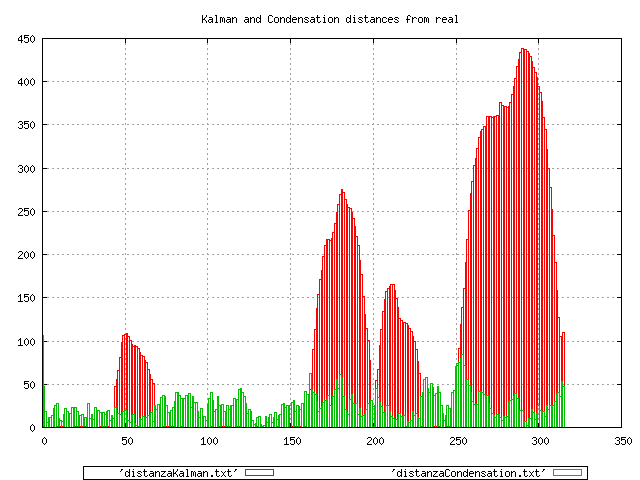
\includegraphics[scale=0.4]{../../esperimenti/movie12/mod_3-Q_1000-S_100/plot-distances.png}
\caption{\textit{Test 4: Previsioni}}
\end{figure}

Statistiche:
\begin{itemize}
\item \begin{math} \bar \delta_K: 105 \end{math}
\item \begin{math} \bar \delta_C: 24 \end{math}
\item \begin{math}(\sigma_x,\sigma_y)\end{math}: (140,92)
\end{itemize}


Di contro con questo test si nota come passando da 1000 a 100 samples invece il risultato sia notevolemente diverso. La stima del moto come si vede dal grafico è notevolemente peggiore nel secondo caso. 
Fortunatamente ha anche poco senso limitare così tanto il numero di samples, mentre un numero molto alto di samples per noi non comporta nessun particolare svantaggio. 

\newpage
\subsubsection{Test 5: MOD=3, Q=1000, S=10}

\begin{figure}[hb]
\centering
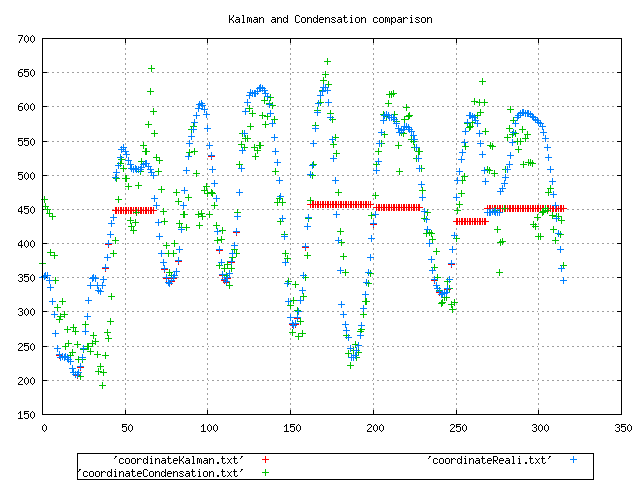
\includegraphics[scale=0.4]{../../esperimenti/movie12/mod_3-Q_1000-S_10/plot.png}
\caption{\textit{Test 5: Tracciamento}}
\end{figure}

\begin{figure}[hb]
\centering
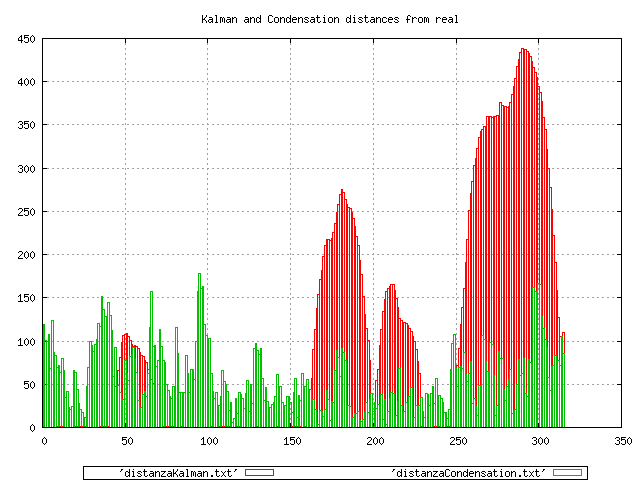
\includegraphics[scale=0.4]{../../esperimenti/movie12/mod_3-Q_1000-S_10/plot-distances.png}
\caption{\textit{Test 5: Previsioni}}
\end{figure}

Statistiche:
\begin{itemize}
\item \begin{math} \bar \delta_K: 105 \end{math}
\item \begin{math} \bar \delta_C: 55 \end{math}
\item \begin{math}(\sigma_x,\sigma_y)\end{math}: (195,112)
\end{itemize}


Abbiamo proseguito nel diminuire il numero di Samples per il Condensation passando a 10, il confronto tra il caso in cui i samples erano 1000 è autoesplicativo: il risultato è notevolemente peggiore. Come ci si poteva aspettare in condizioni estreme di lavoro le previsioni sono decisamente inattendibili.

\newpage
\subsection{Video: tappetonomod.avi}

\begin{itemize}
\item risoluzione: 320x240
\item fps: 10.00
\item durata: 60 s
\end{itemize}

Si tratta di una ripresa trasversale dall'alto. L'oggetto in movimento è un'automobilina radiocomandata che si muove su un'area delimitata da un tappeto. Il moto dell'automobilina subisce repentine accelerazioni e decelerazioni. Non ci sono oggetti occludenti, ma l'automobilina entra ed esce totalmente o parzialmente più di una volta dalla scena.

\begin{figure}[hb]
\centering
	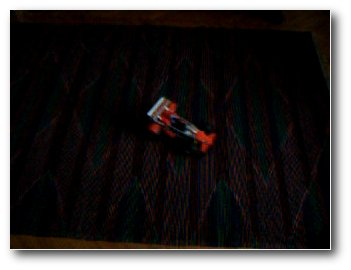
\includegraphics[scale=0.5]{tappeto_nomod.jpg}
\caption{\textit{tappeto-nomod screenshot}}
\end{figure}

\newpage
\subsubsection{Test 6: MOD=3, Q=1000, S=1000}

\begin{figure}[hb]
\centering
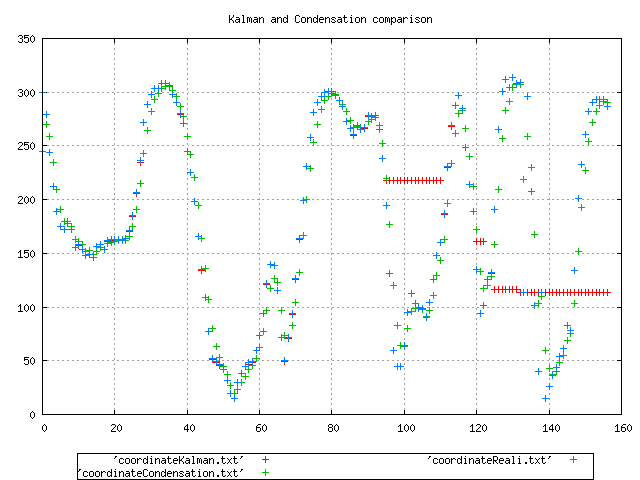
\includegraphics[scale=0.4]{../../esperimenti/tappeto_nozoom/mod_3-Q_1000-S_1000/plot.png}
\caption{\textit{Test 6: Tracciamento}}
\end{figure}

\begin{figure}[hb]
\centering
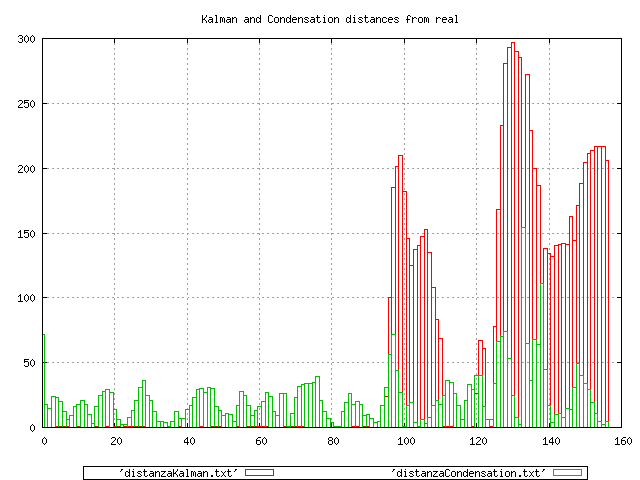
\includegraphics[scale=0.4]{../../esperimenti/tappeto_nozoom/mod_3-Q_1000-S_1000/plot-distances.png}
\caption{\textit{Test 6: Previsioni}}
\end{figure}

Statistiche:
\begin{itemize}
\item \begin{math} \bar \delta_K: 53 \end{math}
\item \begin{math} \bar \delta_C: 22 \end{math}
\item \begin{math}(\sigma_x,\sigma_y)\end{math}: (53,22)
\end{itemize}

La macchinina si sposta in modo molto rapido. Kalman si comporta in modo egregio fintanto che l'oggetto si trova nell'inquadratura e che l'accelerazione della macchina non è tale da far uscire l'oggetto dall'area di previsione. Il Condensation mantiene un buon comportamento anche se mai perfetto.

\newpage
\subsubsection{Test 7: MOD=5, Q=1000, S=1000}

\begin{figure}[hb]
\centering
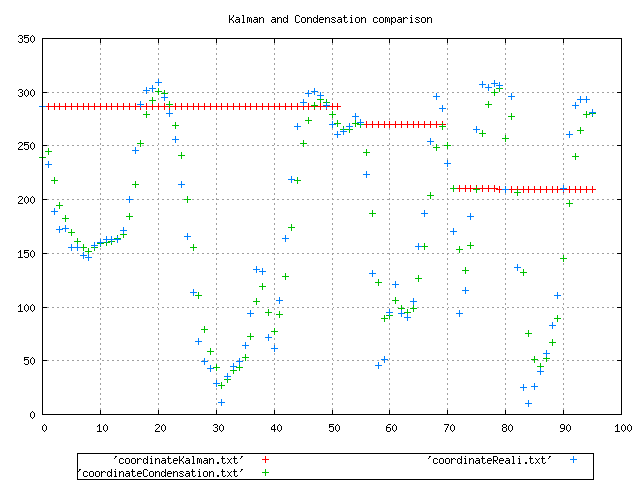
\includegraphics[scale=0.4]{../../esperimenti/tappeto_nozoom/mod_5-Q_1000-S_1000/plot.png}
\caption{\textit{Test 7: Tracciamento}}
\end{figure}

\begin{figure}[hb]
\centering
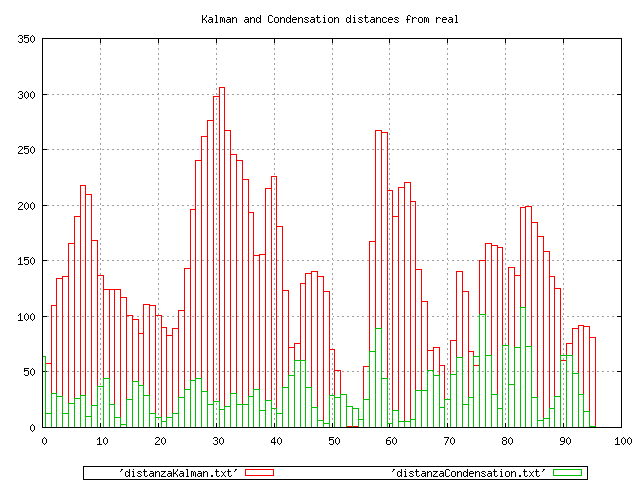
\includegraphics[scale=0.4]{../../esperimenti/tappeto_nozoom/mod_5-Q_1000-S_1000/plot-distances.png}
\caption{\textit{Test 7: Previsioni}}
\end{figure}

Statistiche:
\begin{itemize}
\item \begin{math} \bar \delta_K: 137 \end{math}
\item \begin{math} \bar \delta_C: 31\end{math}
\item \begin{math}(\sigma_x,\sigma_y)\end{math}: (56,40)
\end{itemize} 

Come prevedibile la rapidità di moto di questo oggetto mal si concilia una misurazione effettuata ad intervalli ampi. Entrambi i filtri si comportano in modo non proprio ottimale, in particolare Kalman perde quasi immediatamente l'oggetto. 

\newpage
\subsubsection{Test 8: MOD=2, Q=1000, S=1000}

\begin{figure}[hb]
\centering
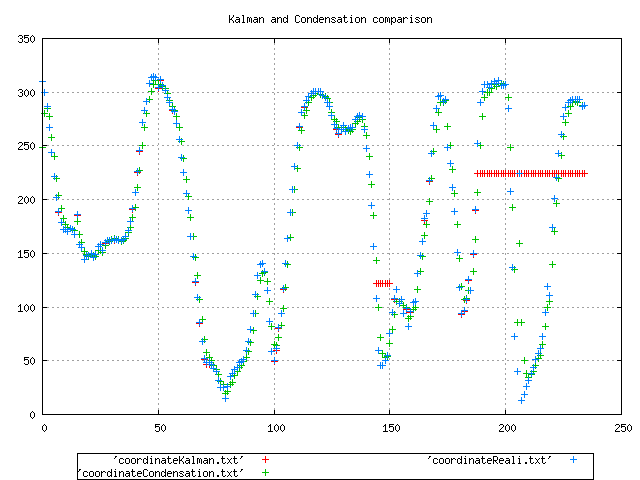
\includegraphics[scale=0.4]{../../esperimenti/tappeto_nozoom/mod_2-Q_1000-S_1000/plot.png}
\caption{\textit{Test 8: Tracciamento}}
\end{figure}

\begin{figure}[hb]
\centering
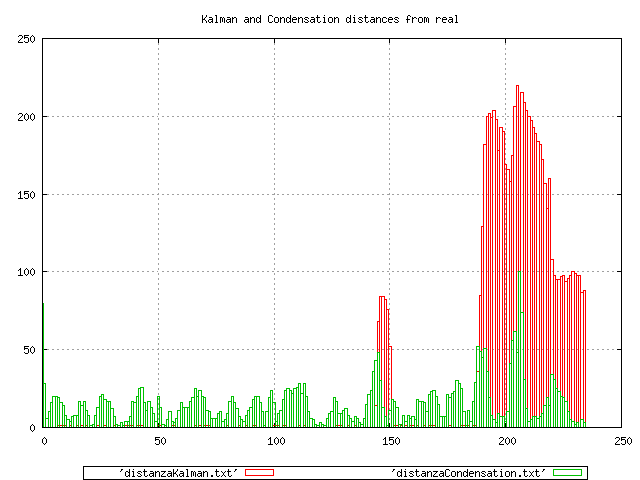
\includegraphics[scale=0.4]{../../esperimenti/tappeto_nozoom/mod_2-Q_1000-S_1000/plot-distances.png}
\caption{\textit{Test 8: Previsioni}}
\end{figure}

Statistiche:
\begin{itemize}
\item \begin{math} \bar \delta_K: 32 \end{math}
\item \begin{math} \bar \delta_C: 15 \end{math}
\item \begin{math}(\sigma_x,\sigma_y)\end{math}: (55,41)
\end{itemize}

La situazione decisamente migliora se invece campioniamo ogni 2 frames. Kalman fintato che non perde l'oggetto si comporta meglio del Condensation, in media però il Condensation risulta migliore.


\newpage
\subsubsection{Test 9: MOD=1, Q=2000, S=1000}

\begin{figure}[hb]
\centering
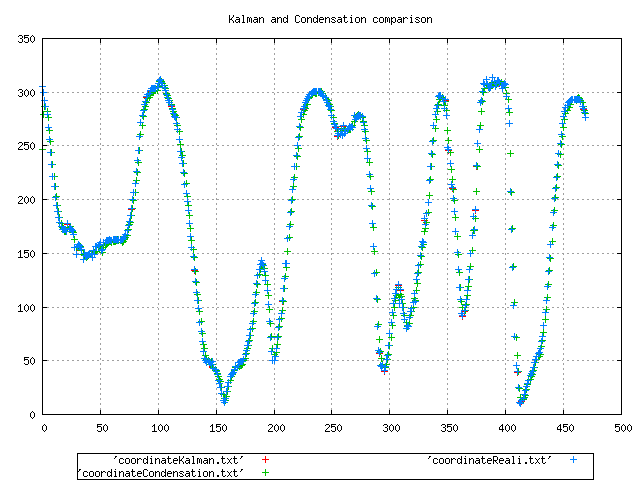
\includegraphics[scale=0.4]{../../esperimenti/tappeto_nozoom/mod_1-Q_2000-S_1000/plot.png}
\caption{\textit{Test 9: Tracciamento}}
\end{figure}

\begin{figure}[hb]
\centering
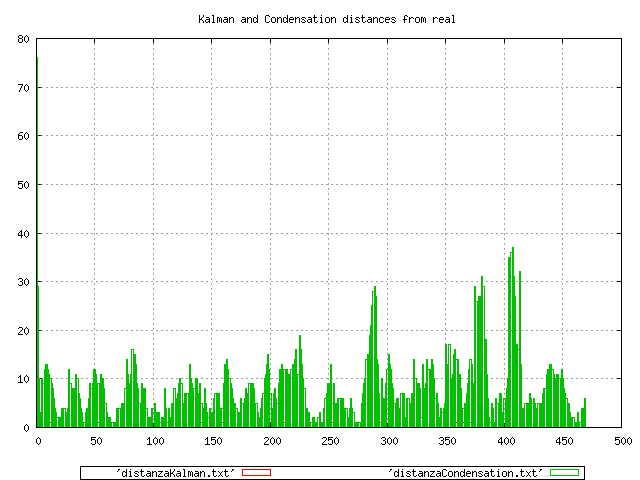
\includegraphics[scale=0.4]{../../esperimenti/tappeto_nozoom/mod_1-Q_2000-S_1000/plot-distances.png}
\caption{\textit{Test 9: Previsioni}}
\end{figure}

Statistiche:
\begin{itemize}
\item \begin{math} \bar \delta_K: 0 \end{math}
\item \begin{math} \bar \delta_C: 8 \end{math}
\item \begin{math}(\sigma_x,\sigma_y)\end{math}: (55,41)
\end{itemize}

Ingrandendo l'area di tolleranza per Kalman e prendendo la misura ogni frame Kalman traccia perfettamente il moto dell'oggetto e anche il Condensation migliora il proprio comportamento. Questa è una situazione ottimale, però decisamente poco realistica. Sono risultati che possiamo ottenere solo perchè stiamo tracciando il moto di un oggetto del quale conosciamo tutto dettagliatamente (Video Stream).

\newpage
\subsubsection{Test 10: MOD=1, Q=500, S=1000}

\begin{figure}[hb]
\centering
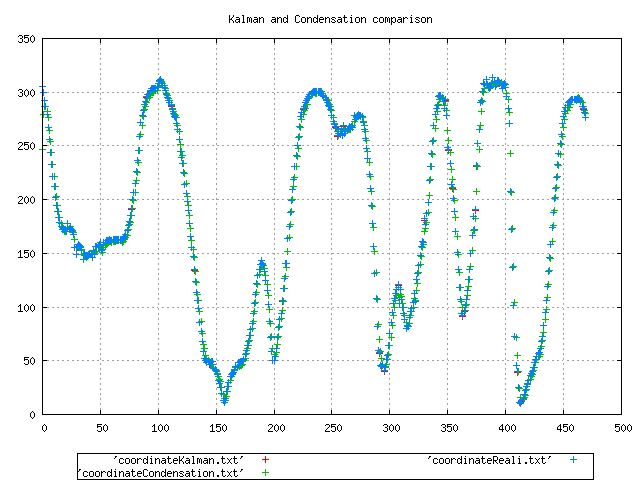
\includegraphics[scale=0.4]{../../esperimenti/tappeto_nozoom/mod_1-Q_500-S_1000/plot.png}
\caption{\textit{Test 10: Tracciamento}}
\end{figure}

\begin{figure}[hb]
\centering
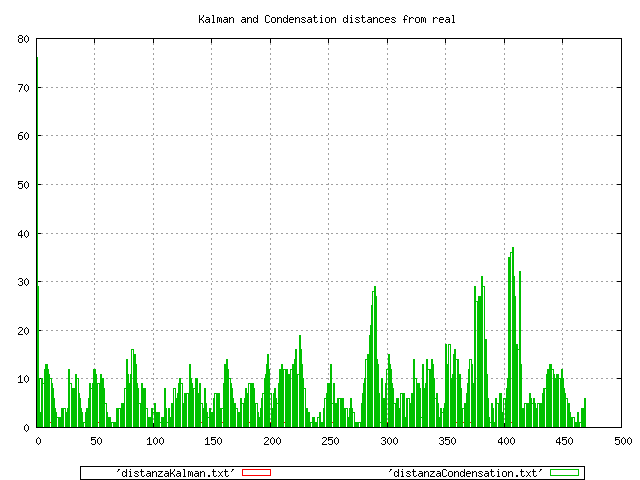
\includegraphics[scale=0.4]{../../esperimenti/tappeto_nozoom/mod_1-Q_500-S_1000/plot-distances.png}
\caption{\textit{Test 10: Previsioni}}
\end{figure}

Statistiche:
\begin{itemize}
\item \begin{math} \bar \delta_K: 0 \end{math}
\item \begin{math} \bar \delta_C: 8 \end{math}
\item \begin{math}(\sigma_x,\sigma_y)\end{math}: (55,41)
\end{itemize}

Campionando ogni frame, anche diminuendo l'area dell'ellisse di tolleranza per Kalman i risultati non cambiano.

\newpage
\subsection{Video: singlecar.avi}

\begin{itemize}
\item risoluzione: 648x484
\item fps: 30.00
\item durata: 33 s
\end{itemize}

Anche in questo caso il video è di un'automobilina radiocomadata ripresa dall'alto trasversalmente. A differenza che negli altri video non ci sono oggetti occludenti e il moto è piuttosto uniforme. L'automobilina, però, entra ed esce dalla scena più di una volta.

\begin{figure}[hb]
\centering
	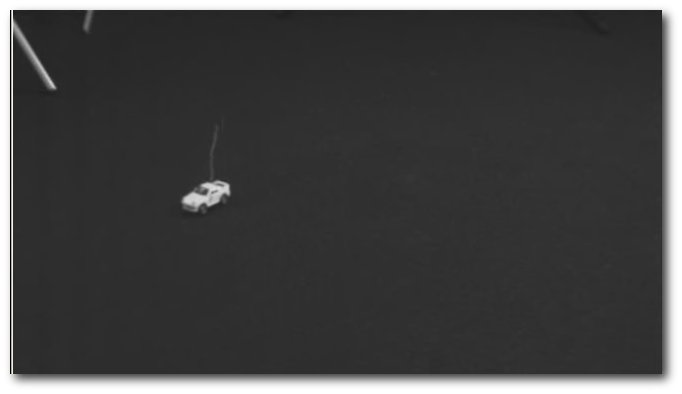
\includegraphics[scale=0.5]{singlecar.jpg}
\caption{\textit{movie12 screenshot}}
\end{figure}

\newpage
\subsubsection{Test 11: MOD=3, Q=1000, S=1000}

\begin{figure}[hb]
\centering
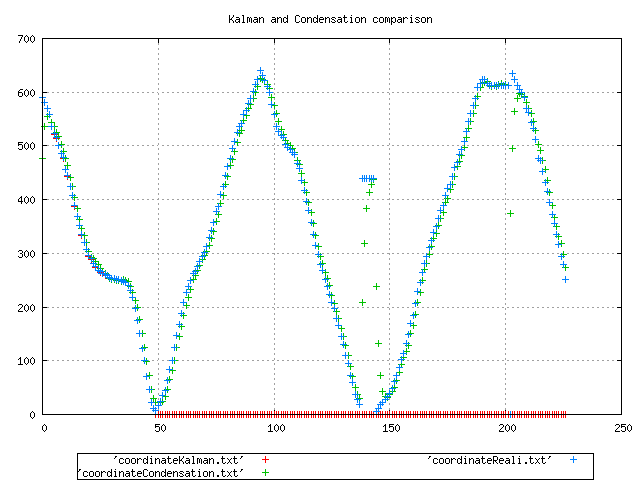
\includegraphics[scale=0.4]{../../esperimenti/single_car/mod_3-Q_1000-S_1000/plot.png}
\caption{\textit{Test 11: Tracciamento}}
\end{figure}

\begin{figure}[hb]
\centering
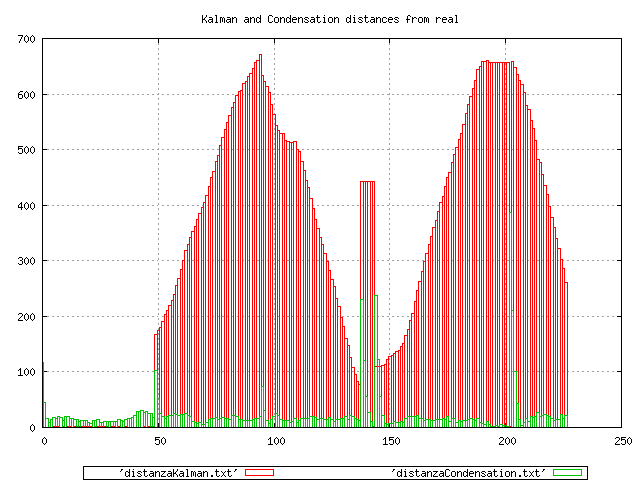
\includegraphics[scale=0.4]{../../esperimenti/single_car/mod_3-Q_1000-S_1000/plot-distances.png}
\caption{\textit{Test 11: Previsioni}}
\end{figure}

Statistiche:
\begin{itemize}
\item \begin{math} \bar \delta_K: 323  \end{math}
\item \begin{math} \bar \delta_C: 23 \end{math}
\item \begin{math}(\sigma_x,\sigma_y)\end{math}: (111,83)
\end{itemize}

In questo test si hanno i risultati più comuni: se l'oggetto scompare dalle scena e riappare in punti molto distanti da dove è scomparso il filtro di Kalman lo perde, ma quando l'oggetto è individuato correttamente Kalman è migliore del Condensation. 
Tuttavia in media il Condensation è molto più preciso nella predizione.

\newpage
\subsubsection{Test 12: MOD=10, Q=5000, S=1000}

\begin{figure}[hb]
\centering
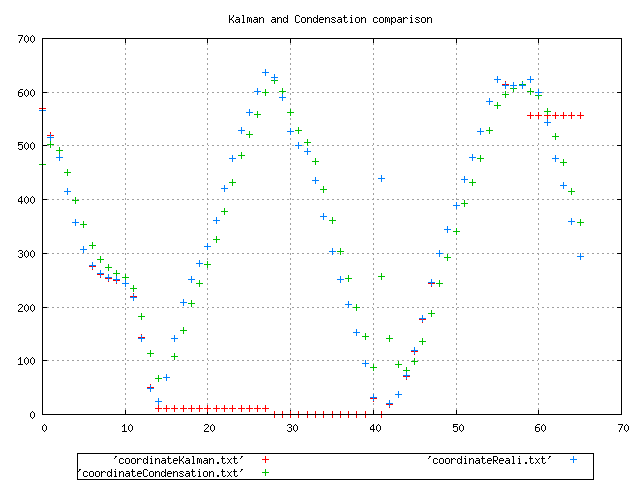
\includegraphics[scale=0.4]{../../esperimenti/single_car/mod_10-Q_5000-S_1000/plot.png}
\caption{\textit{Test 12: Tracciamento}}
\end{figure}

\begin{figure}[hb]
\centering
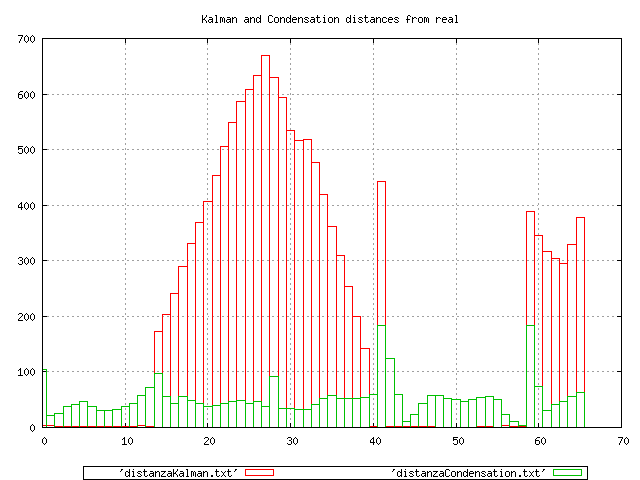
\includegraphics[scale=0.4]{../../esperimenti/single_car/mod_10-Q_5000-S_1000/plot-distances.png}
\caption{\textit{Test 12: Previsioni}}
\end{figure}

Statistiche:
\begin{itemize}
\item \begin{math} \bar \delta_K:  209 \end{math}
\item \begin{math} \bar \delta_C:  52 \end{math}
\item \begin{math}(\sigma_x,\sigma_y)\end{math}: (114,83)
\end{itemize}

Il video in questione si presta ad un tracciamento effettuato ad intervalli anche ampi poichè non ci sono brusche accelerazioni o frenate. Il problema principale sul filtro di Kalman resta che perde l'oggetto se scompare ed è perciò evidente la necessità di incrementare l'area di tolleranza per migliorare le prestazioni del filtro. 

\newpage
\subsubsection{Test 13: MOD=6, Q=1000, S=1000}

\begin{figure}[hb]
\centering
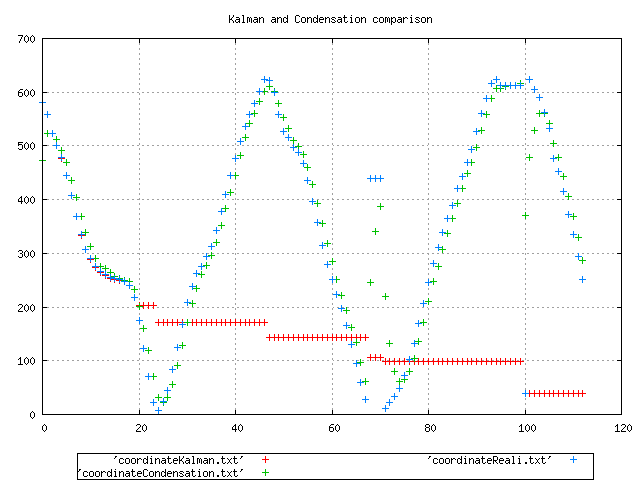
\includegraphics[scale=0.4]{../../esperimenti/single_car/mod_6-Q_1000-S_1000/plot.png}
\caption{\textit{Test 13: Tracciamento}}
\end{figure}

\begin{figure}[hb]
\centering
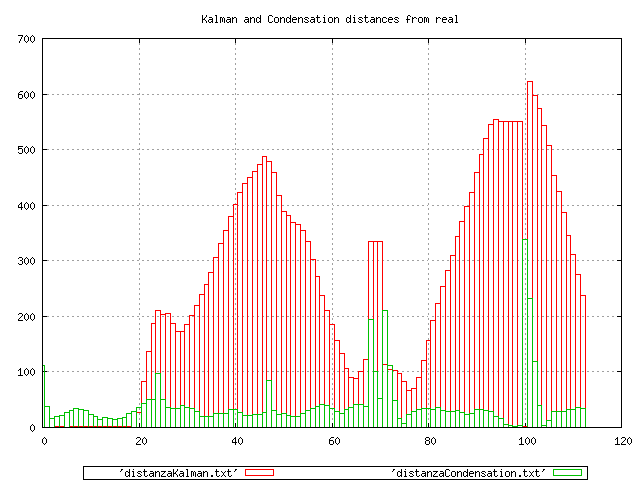
\includegraphics[scale=0.4]{../../esperimenti/single_car/mod_6-Q_1000-S_1000/plot-distances.png}
\caption{\textit{Test 13: Previsioni}}
\end{figure}

Statistiche:
\begin{itemize}
\item \begin{math} \bar \delta_K: 252 \end{math}
\item \begin{math} \bar \delta_C: 40 \end{math}
\item \begin{math}(\sigma_x,\sigma_y)\end{math}: (113,82)
\end{itemize}

Anche riducendo in numero di frames di campionamento la situazione non cambia molto, anzi per un caso crediamo dovuto alla natura del video stesso la situazione addirittura peggiora per il filtro di Kalman.
Decidiamo perciò di togliere il controllo sulla correttezza del rilevamento da parte di Kalman e ci poniamo come unico obiettivo quello di farlo lavorare in condizioni di minima tolleranza sull'errore.

\newpage
\subsubsection{Test 14: MOD=6, Q=1, S=1000}

\begin{figure}[hb]
\centering
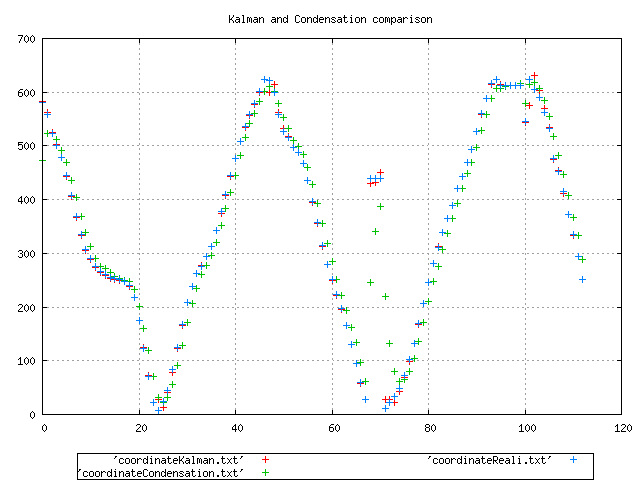
\includegraphics[scale=0.4]{../../esperimenti/single_car/mod_6-Q_1-S_1000/plot.png}
\caption{\textit{Test 14: Tracciamento}}
\end{figure}

\begin{figure}[hb]
\centering
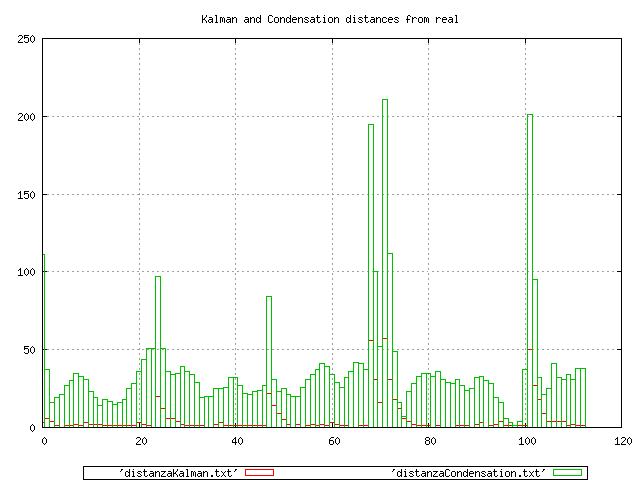
\includegraphics[scale=0.4]{../../esperimenti/single_car/mod_6-Q_1-S_1000/plot-distances.png}
\caption{\textit{Test 14: Previsioni}}
\end{figure}

Statistiche:
\begin{itemize}
\item \begin{math} \bar \delta_K: 5 \end{math}
\item \begin{math} \bar \delta_C: 37 \end{math}
\item \begin{math}(\sigma_x,\sigma_y)\end{math}: (113,82)
\end{itemize}

Togliendo il controllo sulla correttezza della predizione da parte di Kalman, se l'oggetto scompare siamo comuque in grado di tracciarlo (il filtro di Kalman lo ``insegue''). In media Kalman sbaglia pochissimo, il tracciamento è quasi perfetto.
L'obiettivo è ora quello di metterci in una situazione ipotetica in cui Kalman si comporta peggio del Condensation.

\newpage
\subsubsection{Test 15: MOD=6, Q=0.1, S=1000}

\begin{figure}[hb]
\centering
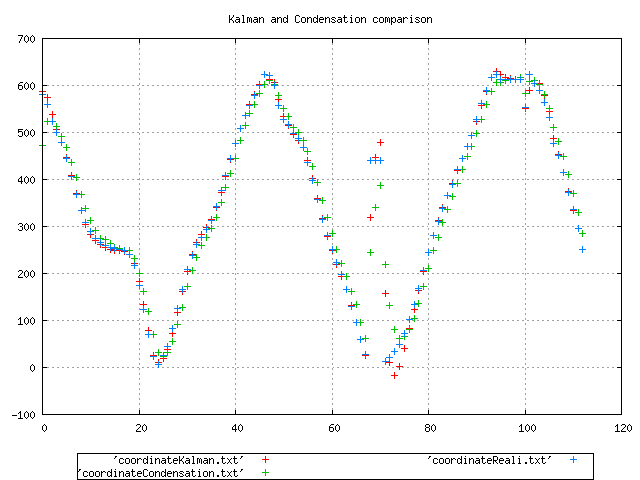
\includegraphics[scale=0.4]{../../esperimenti/single_car/mod_6-Q_0.1-S_1000/plot.png}
\caption{\textit{Test 15: Tracciamento}}
\end{figure}

\begin{figure}[hb]
\centering
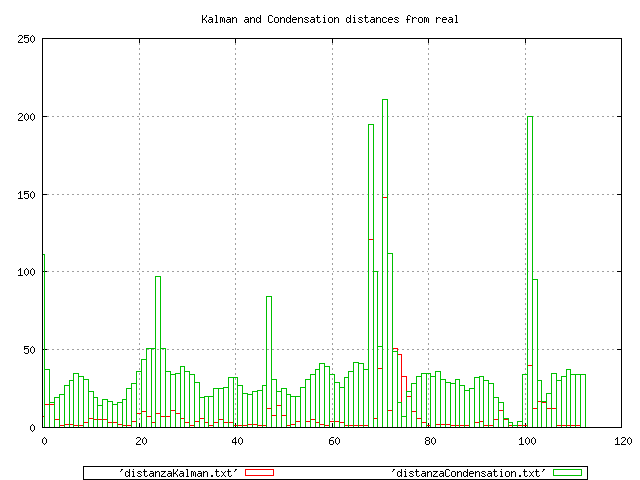
\includegraphics[scale=0.4]{../../esperimenti/single_car/mod_6-Q_0.1-S_1000/plot-distances.png}
\caption{\textit{Test 15: Previsioni}}
\end{figure}

Statistiche:
\begin{itemize}
\item \begin{math} \bar \delta_K: 8 \end{math}
\item \begin{math} \bar \delta_C: 37 \end{math}
\item \begin{math}(\sigma_x,\sigma_y)\end{math}: (113,82)
\end{itemize}

Riduciamo l'errore consentito sulla predizione, l'ellisse di tolleranza si riduce imponendo a Kalma di sbagliare il meno possibile. In questo test i risultati ottenuti non si discostano molto da quelli precedenti, l'oggetto è sempre tracciato ottimamente dal filtro di Kalman.

\newpage
\subsubsection{Test 16: MOD=6, Q=0.001, S=1000}

\begin{figure}[hb]
\centering
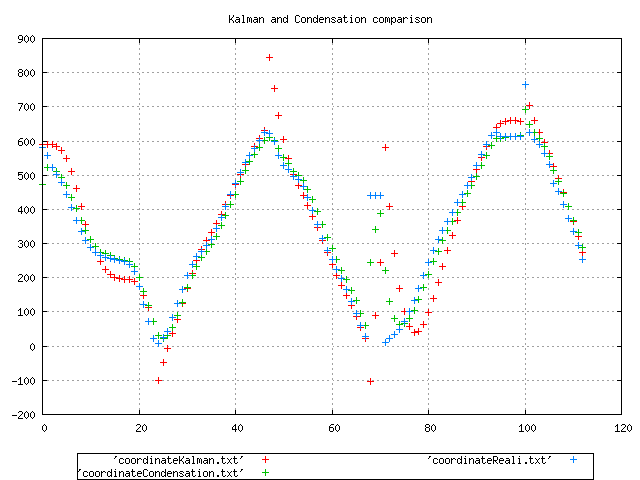
\includegraphics[scale=0.4]{../../esperimenti/single_car/mod_6-Q_0.001-S_1000/plot.png}
\caption{\textit{Test 16: Tracciamento}}
\end{figure}

\begin{figure}[hb]
\centering
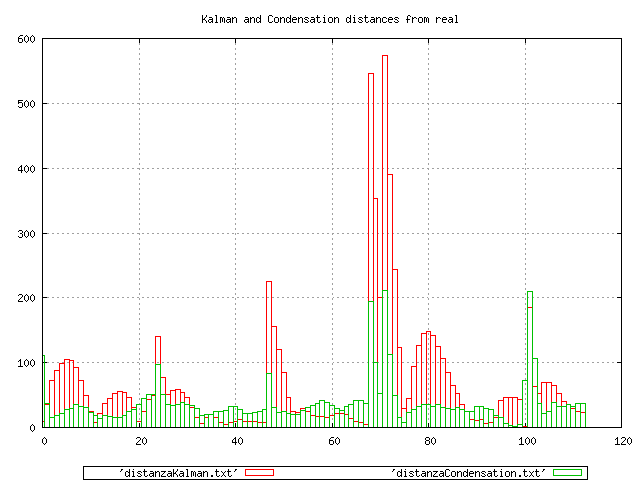
\includegraphics[scale=0.4]{../../esperimenti/single_car/mod_6-Q_0.001-S_1000/plot-distances.png}
\caption{\textit{Test 16: Previsioni}}
\end{figure}

Statistiche:
\begin{itemize}
\item \begin{math} \bar \delta_K: 66 \end{math}
\item \begin{math} \bar \delta_C: 43 \end{math}
\item \begin{math}(\sigma_x,\sigma_y)\end{math}: (114,82)
\end{itemize}

Come previsto il filtro di Kalman comincia finalmente a peggiorare il proprio comportamento anche se in media è sempre migliore dell'altro. 

\newpage
\subsubsection{Test 17: MOD=6, Q=0.0001, S=1000}

\begin{figure}[hb]
\centering
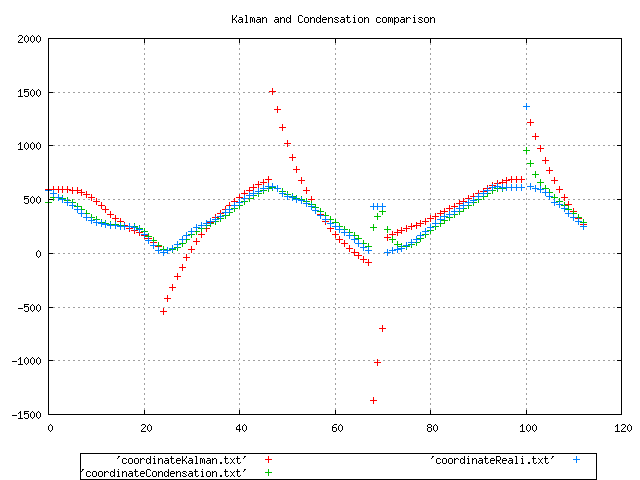
\includegraphics[scale=0.4]{../../esperimenti/single_car/mod_6-Q_0.0001-S_1000/plot.png}
\caption{\textit{Test 17: Tracciamento}}
\end{figure}

\begin{figure}[hb]
\centering
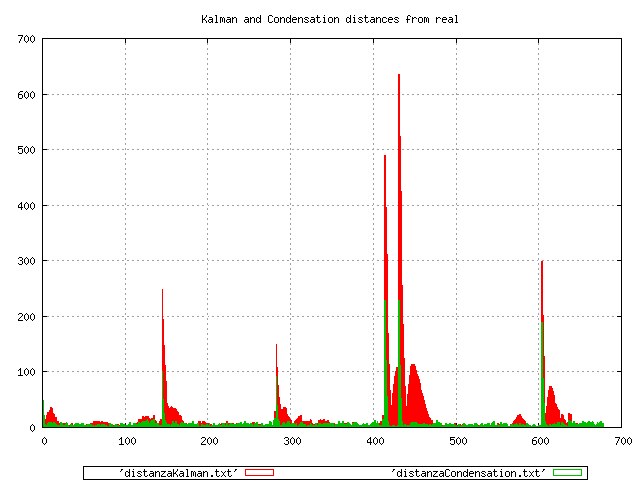
\includegraphics[scale=0.4]{../../esperimenti/single_car/mod_1-Q_0.0001-S_1000/plot-distances.png}
\caption{\textit{Test 17: Previsioni}}
\end{figure}

Statistiche:
\begin{itemize}
\item \begin{math} \bar \delta_K: 179 \end{math}
\item \begin{math} \bar \delta_C: 43 \end{math}
\item \begin{math}(\sigma_x,\sigma_y)\end{math}: (114,83)
\end{itemize}

In questo test Kalman non riesce più a tracciare correttamente l'oggetto. Appare qui evidente come alcune zone si dimostrino particolarmente critiche per il filtro di Kalman.

\newpage
\subsubsection{Test 18: MOD=1, Q=0.0001, S=1000}

\begin{figure}[hb]
\centering
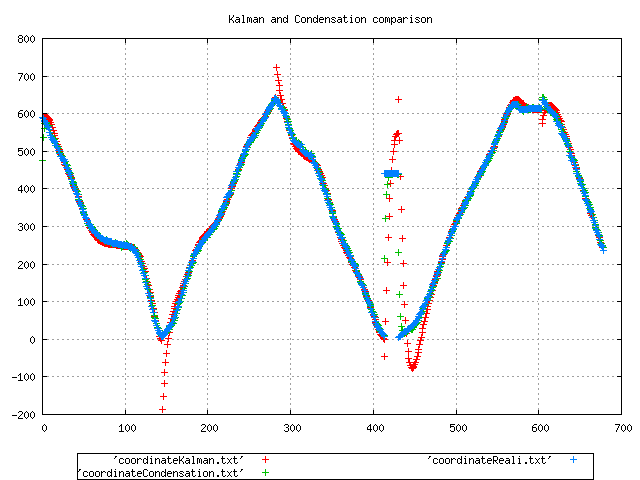
\includegraphics[scale=0.4]{../../esperimenti/single_car/mod_1-Q_0.0001-S_1000/plot.png}
\caption{\textit{Test 18: Tracciamento}}
\end{figure}

\begin{figure}[hb]
\centering
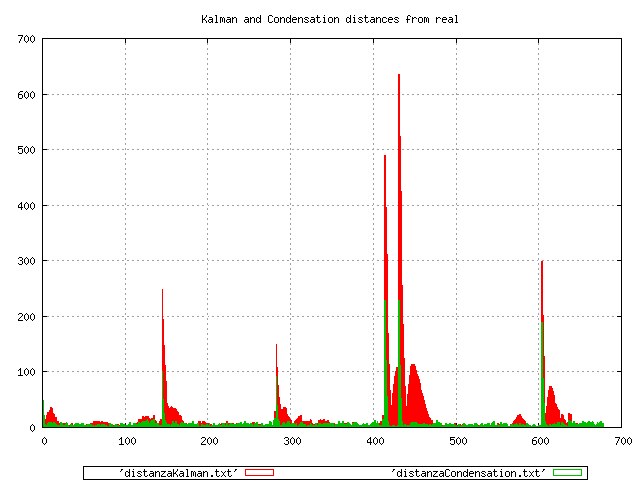
\includegraphics[scale=0.4]{../../esperimenti/single_car/mod_1-Q_0.0001-S_1000/plot-distances.png}
\caption{\textit{Test 18: Previsioni}}
\end{figure}

Abbiamo variato anche la frequenza di campionamento.
Qui il comportamento di Kalman è migliore rispetto al test precedente ed è più chiaro come Kalman si trovi in difficoltà soprattutto nel tracciare zone di non linearità del moto dell'oggetto. (smoothness)

Statistiche:
\begin{itemize}
\item \begin{math} \bar \delta_K: 22 \end{math}
\item \begin{math} \bar \delta_C: 8\end{math}
\item \begin{math}(\sigma_x,\sigma_y)\end{math}: (111,85)
\end{itemize}


 \chapter{Conclusioni}

Con questo elaborato si è voluto differenziare nel primo capitolo i concetti di Proprietà Intellettuale e Industriale, che pur rimanendo molto simili, nascono da un sostrato abbastanza diverso, anche se rispettivamente la prima copre una serie di diritti maggiore della seconda, come riportato nella visione insiemistica in figura \ref{fig:PI} . I tipi di tutela quindi che derivano da entrambi sono leggermente diversi in quanto il primo si attaglia al diritto d'autore in generale e l'altro alla tutela dell'invenzione come prodotto industriale. Fatto questo si è passati a definire brevemente il concetto di copyright, dilungandosi invece leggermente nella descrizione dei brevetti e marchi, forme di tutela della Proprietà Intellettuale, in quanto più coerenti con la traccia della trattazione.

Il capitolo secondo si contraddistingue perché, dopo aver data la definizione di brevetto, entra nel merito di tutta la trattazione: la tutela del software attraverso lo strumento del brevetto. Su questo concetto emergono tutt'oggi pareri contrastanti, per questo motivo la trattazione si è fatta molto interessante. Si è percorso un breve excursus sulla tutela giuridica del software secondo copyright, successivamente si è riassunto la storia dei brevetti software in UE e in USA, dandone una visione dall'alto e riportando i casi giuridici principali di ogni paese.

La trattazione poi si è spostata su tempi più recenti e ambiti tecnici. In particolare nel capitolo terzo si è osservato il tagliente punto di vista della Free Software Foundation nei confronti dei software patens, legati anche ad altre tecnologie recenti di restrizione dei diritti degli utenti. Si è quindi analizzato i nuovi articoli che compongono la nuova licenza copyleft: la GNU General Public License versione 3.
Infine si è dato un esempio degli effetti provati da questa, nella distribuzione del software gplv3 con software house che hanno sottoscritto patents agreement con altre lampante in questo è il caso Novell-Microsoft e il passaggio di licenza del software di interoperabilità tra reti Samba.

Ricordando di dare una veste pratica oltre che legale, l'ultimo capitolo prende come esempio il brevetto del formato di compressione audio per antonomasia, cioè l'mp3: il brevetto non è unico, ma sono una serie di brevetti detenuti da molte società; è stato quindi effettuato un lungo lavoro per districarsi nella rete brevettuale che si è formata. Prendendo questo caso, si vuole mostrare quali sono gli effetti della brevettazione, della difficoltà legata alla eterogeneità delle varie legislazioni e degli effetti apportate al free software o a software house commerciali.

Dalla trattazione è quindi emerso che il software è giusto che venga tutelato dal diritto d'autore; è anche vero d'altro canto che non può essere concepito solo come una mera composizione logico-intellettuale, visto l'enorme commercio del mercato del software. E quindi in questo senso è giusto affermare che anche il software,pur rimanendo un bene immateriale diverso dall'hardware, è entrato nella schiera dei prodotti industriali a tutti gli effetti. Appurato questo è giusto chiedersi se è lecito lasciare il software sotto copyright o addirittura applicare la nozione di brevetto, concepita per prodotti fisici o processi industriali, anche agli algoritmi implementati. Oppure invece notando l'uso che poi ne viene fatto dalle software house, potrebbe essere possibile negare l'applicazione del brevetto al software, in maniera congrua con quanto affermato dalla Free Software Foundation nella GPLv3, magari trovando una via alternativa tra la tutela intellettuale troppo generica e la tutela industriale troppo legata al monopolio.


\bibliographystyle{IEEEtran}
\bibliography{bibliografia}



\end{document} 